% REV01 Sun 27 Jun 2021 12:08:33 WIB
% START Tue 04 May 2021 13:55:16 WIB

\chapter{A CRY FOR HELP}

The Paper Mill had stopped work for the night, and the paths and roads
in its neighbourhood were sprinkled with clusters of people going home
from their day’s labour in it. There were men, women, and children in
the groups, and there was no want of lively colour to flutter in the
gentle evening wind. The mingling of various voices and the sound of
laughter made a cheerful impression upon the ear, analogous to that of
the fluttering colours upon the eye. Into the sheet of water reflecting
the flushed sky in the foreground of the living picture, a knot of
urchins were casting stones, and watching the expansion of the rippling
circles. So, in the rosy evening, one might watch the ever-widening
beauty of the landscape--beyond the newly-released workers wending
home--beyond the silver river--beyond the deep green fields of corn, so
prospering, that the loiterers in their narrow threads of pathway seemed
to float immersed breast-high--beyond the hedgerows and the clumps of
trees--beyond the windmills on the ridge--away to where the sky appeared
to meet the earth, as if there were no immensity of space between
mankind and Heaven.

It was a Saturday evening, and at such a time the village dogs, always
much more interested in the doings of humanity than in the affairs of
their own species, were particularly active. At the general shop, at
the butcher’s and at the public-house, they evinced an inquiring spirit
never to be satiated. Their especial interest in the public-house would
seem to imply some latent rakishness in the canine character; for little
was eaten there, and they, having no taste for beer or tobacco (Mrs
Hubbard’s dog is said to have smoked, but proof is wanting), could only
have been attracted by sympathy with loose convivial habits. Moreover,
a most wretched fiddle played within; a fiddle so unutterably vile, that
one lean long-bodied cur, with a better ear than the rest, found himself
under compulsion at intervals to go round the corner and howl. Yet, even
he returned to the public-house on each occasion with the tenacity of a
confirmed drunkard.

Fearful to relate, there was even a sort of little Fair in the village.
Some despairing gingerbread that had been vainly trying to dispose of
itself all over the country, and had cast a quantity of dust upon its
head in its mortification, again appealed to the public from an infirm
booth. So did a heap of nuts, long, long exiled from Barcelona, and yet
speaking English so indifferently as to call fourteen of themselves
a pint. A Peep-show which had originally started with the Battle of
Waterloo, and had since made it every other battle of later date
by altering the Duke of Wellington’s nose, tempted the student of
illustrated history. A Fat Lady, perhaps in part sustained upon
postponed pork, her professional associate being a Learned Pig,
displayed her life-size picture in a low dress as she appeared when
presented at Court, several yards round. All this was a vicious
spectacle as any poor idea of amusement on the part of the rougher
hewers of wood and drawers of water in this land of England ever is and
shall be. They MUST NOT vary the rheumatism with amusement. They may
vary it with fever and ague, or with as many rheumatic variations as
they have joints; but positively not with entertainment after their own
manner.

The various sounds arising from this scene of depravity, and floating
away into the still evening air, made the evening, at any point which
they just reached fitfully, mellowed by the distance, more still by
contrast. Such was the stillness of the evening to Eugene Wrayburn, as
he walked by the river with his hands behind him.

He walked slowly, and with the measured step and preoccupied air of one
who was waiting. He walked between the two points, an osier-bed at this
end and some floating lilies at that, and at each point stopped and
looked expectantly in one direction.

‘It is very quiet,’ said he.

It was very quiet. Some sheep were grazing on the grass by the
river-side, and it seemed to him that he had never before heard the
crisp tearing sound with which they cropped it. He stopped idly, and
looked at them.

‘You are stupid enough, I suppose. But if you are clever enough to get
through life tolerably to your satisfaction, you have got the better of
me, Man as I am, and Mutton as you are!’

A rustle in a field beyond the hedge attracted his attention. ‘What’s
here to do?’ he asked himself leisurely going towards the gate and
looking over. ‘No jealous paper-miller? No pleasures of the chase in
this part of the country? Mostly fishing hereabouts!’

The field had been newly mown, and there were yet the marks of the
scythe on the yellow-green ground, and the track of wheels where the hay
had been carried. Following the tracks with his eyes, the view closed
with the new hayrick in a corner.

Now, if he had gone on to the hayrick, and gone round it? But, say
that the event was to be, as the event fell out, and how idle are such
suppositions! Besides, if he had gone; what is there of warning in a
Bargeman lying on his face?

‘A bird flying to the hedge,’ was all he thought about it; and came
back, and resumed his walk.

‘If I had not a reliance on her being truthful,’ said Eugene, after
taking some half-dozen turns, ‘I should begin to think she had given me
the slip for the second time. But she promised, and she is a girl of her
word.’

Turning again at the water-lilies, he saw her coming, and advanced to
meet her.

‘I was saying to myself, Lizzie, that you were sure to come, though you
were late.’

‘I had to linger through the village as if I had no object before me,
and I had to speak to several people in passing along, Mr Wrayburn.’

‘Are the lads of the village--and the ladies--such scandal-mongers?’ he
asked, as he took her hand and drew it through his arm.

She submitted to walk slowly on, with downcast eyes. He put her hand to
his lips, and she quietly drew it away.

‘Will you walk beside me, Mr Wrayburn, and not touch me?’ For, his arm
was already stealing round her waist.

She stopped again, and gave him an earnest supplicating look. ‘Well,
Lizzie, well!’ said he, in an easy way though ill at ease with himself
‘don’t be unhappy, don’t be reproachful.’

‘I cannot help being unhappy, but I do not mean to be reproachful. Mr
Wrayburn, I implore you to go away from this neighbourhood, to-morrow
morning.’

‘Lizzie, Lizzie, Lizzie!’ he remonstrated. ‘As well be reproachful as
wholly unreasonable. I can’t go away.’

‘Why not?’

‘Faith!’ said Eugene in his airily candid manner. ‘Because you won’t let
me. Mind! I don’t mean to be reproachful either. I don’t complain that
you design to keep me here. But you do it, you do it.’

‘Will you walk beside me, and not touch me;’ for, his arm was coming
about her again; ‘while I speak to you very seriously, Mr Wrayburn?’

‘I will do anything within the limits of possibility, for you, Lizzie,’
he answered with pleasant gaiety as he folded his arms. ‘See here!
Napoleon Buonaparte at St Helena.’

‘When you spoke to me as I came from the Mill the night before last,’
said Lizzie, fixing her eyes upon him with the look of supplication
which troubled his better nature, ‘you told me that you were much
surprised to see me, and that you were on a solitary fishing excursion.
Was it true?’

‘It was not,’ replied Eugene composedly, ‘in the least true. I came
here, because I had information that I should find you here.’

‘Can you imagine why I left London, Mr Wrayburn?’

‘I am afraid, Lizzie,’ he openly answered, ‘that you left London to get
rid of me. It is not flattering to my self-love, but I am afraid you
did.’

‘I did.’

‘How could you be so cruel?’

‘O Mr Wrayburn,’ she answered, suddenly breaking into tears, ‘is the
cruelty on my side! O Mr Wrayburn, Mr Wrayburn, is there no cruelty in
your being here to-night!’

‘In the name of all that’s good--and that is not conjuring you in my
own name, for Heaven knows I am not good’--said Eugene, ‘don’t be
distressed!’

‘What else can I be, when I know the distance and the difference between
us? What else can I be, when to tell me why you came here, is to put me
to shame!’ said Lizzie, covering her face.

He looked at her with a real sentiment of remorseful tenderness and
pity. It was not strong enough to impell him to sacrifice himself and
spare her, but it was a strong emotion.

‘Lizzie! I never thought before, that there was a woman in the world who
could affect me so much by saying so little. But don’t be hard in your
construction of me. You don’t know what my state of mind towards you is.
You don’t know how you haunt me and bewilder me. You don’t know how the
cursed carelessness that is over-officious in helping me at every other
turning of my life, WON’T help me here. You have struck it dead, I
think, and I sometimes almost wish you had struck me dead along with
it.’

She had not been prepared for such passionate expressions, and they
awakened some natural sparks of feminine pride and joy in her breast. To
consider, wrong as he was, that he could care so much for her, and that
she had the power to move him so!

‘It grieves you to see me distressed, Mr Wrayburn; it grieves me to see
you distressed. I don’t reproach you. Indeed I don’t reproach you.
You have not felt this as I feel it, being so different from me, and
beginning from another point of view. You have not thought. But I
entreat you to think now, think now!’

‘What am I to think of?’ asked Eugene, bitterly.

‘Think of me.’

‘Tell me how NOT to think of you, Lizzie, and you’ll change me
altogether.’

‘I don’t mean in that way. Think of me, as belonging to another station,
and quite cut off from you in honour. Remember that I have no protector
near me, unless I have one in your noble heart. Respect my good name.
If you feel towards me, in one particular, as you might if I was a lady,
give me the full claims of a lady upon your generous behaviour. I am
removed from you and your family by being a working girl. How true a
gentleman to be as considerate of me as if I was removed by being a
Queen!’

He would have been base indeed to have stood untouched by her appeal.
His face expressed contrition and indecision as he asked:

‘Have I injured you so much, Lizzie?’

‘No, no. You may set me quite right. I don’t speak of the past, Mr
Wrayburn, but of the present and the future. Are we not here now,
because through two days you have followed me so closely where there
are so many eyes to see you, that I consented to this appointment as an
escape?’

‘Again, not very flattering to my self-love,’ said Eugene, moodily; ‘but
yes. Yes. Yes.’

‘Then I beseech you, Mr Wrayburn, I beg and pray you, leave this
neighbourhood. If you do not, consider to what you will drive me.’

He did consider within himself for a moment or two, and then retorted,
‘Drive you? To what shall I drive you, Lizzie?’

‘You will drive me away. I live here peacefully and respected, and I am
well employed here. You will force me to quit this place as I quitted
London, and--by following me again--will force me to quit the next place
in which I may find refuge, as I quitted this.’

‘Are you so determined, Lizzie--forgive the word I am going to use, for
its literal truth--to fly from a lover?’

‘I am so determined,’ she answered resolutely, though trembling, ‘to fly
from such a lover. There was a poor woman died here but a little while
ago, scores of years older than I am, whom I found by chance, lying on
the wet earth. You may have heard some account of her?’

‘I think I have,’ he answered, ‘if her name was Higden.’

‘Her name was Higden. Though she was so weak and old, she kept true to
one purpose to the very last. Even at the very last, she made me promise
that her purpose should be kept to, after she was dead, so settled
was her determination. What she did, I can do. Mr Wrayburn, if I
believed--but I do not believe--that you could be so cruel to me as
to drive me from place to place to wear me out, you should drive me to
death and not do it.’

He looked full at her handsome face, and in his own handsome face there
was a light of blended admiration, anger, and reproach, which she--who
loved him so in secret whose heart had long been so full, and he the
cause of its overflowing--drooped before. She tried hard to retain her
firmness, but he saw it melting away under his eyes. In the moment of
its dissolution, and of his first full knowledge of his influence upon
her, she dropped, and he caught her on his arm.

‘Lizzie! Rest so a moment. Answer what I ask you. If I had not been what
you call removed from you and cut off from you, would you have made this
appeal to me to leave you?’

‘I don’t know, I don’t know. Don’t ask me, Mr Wrayburn. Let me go back.’

‘I swear to you, Lizzie, you shall go directly. I swear to you, you
shall go alone. I’ll not accompany you, I’ll not follow you, if you will
reply.’

‘How can I, Mr Wrayburn? How can I tell you what I should have done, if
you had not been what you are?’

‘If I had not been what you make me out to be,’ he struck in, skilfully
changing the form of words, ‘would you still have hated me?’

‘O Mr Wrayburn,’ she replied appealingly, and weeping, ‘you know me
better than to think I do!’

‘If I had not been what you make me out to be, Lizzie, would you still
have been indifferent to me?’

‘O Mr Wrayburn,’ she answered as before, ‘you know me better than that
too!’

There was something in the attitude of her whole figure as he supported
it, and she hung her head, which besought him to be merciful and not
force her to disclose her heart. He was not merciful with her, and he
made her do it.

‘If I know you better than quite to believe (unfortunate dog though I
am!) that you hate me, or even that you are wholly indifferent to me,
Lizzie, let me know so much more from yourself before we separate. Let
me know how you would have dealt with me if you had regarded me as being
what you would have considered on equal terms with you.’

‘It is impossible, Mr Wrayburn. How can I think of you as being on equal
terms with me? If my mind could put you on equal terms with me, you
could not be yourself. How could I remember, then, the night when I
first saw you, and when I went out of the room because you looked at
me so attentively? Or, the night that passed into the morning when you
broke to me that my father was dead? Or, the nights when you used to
come to see me at my next home? Or, your having known how uninstructed
I was, and having caused me to be taught better? Or, my having so looked
up to you and wondered at you, and at first thought you so good to be at
all mindful of me?’

‘Only “at first” thought me so good, Lizzie? What did you think me after
“at first”? So bad?’

‘I don’t say that. I don’t mean that. But after the first wonder and
pleasure of being noticed by one so different from any one who had ever
spoken to me, I began to feel that it might have been better if I had
never seen you.’

‘Why?’

‘Because you WERE so different,’ she answered in a lower voice. ‘Because
it was so endless, so hopeless. Spare me!’

‘Did you think for me at all, Lizzie?’ he asked, as if he were a little
stung.

‘Not much, Mr Wrayburn. Not much until to-night.’

‘Will you tell me why?’

‘I never supposed until to-night that you needed to be thought for. But
if you do need to be; if you do truly feel at heart that you have indeed
been towards me what you have called yourself to-night, and that there
is nothing for us in this life but separation; then Heaven help you, and
Heaven bless you!’

The purity with which in these words she expressed something of her
own love and her own suffering, made a deep impression on him for the
passing time. He held her, almost as if she were sanctified to him by
death, and kissed her, once, almost as he might have kissed the dead.

‘I promised that I would not accompany you, nor follow you. Shall I keep
you in view? You have been agitated, and it’s growing dark.’

‘I am used to be out alone at this hour, and I entreat you not to do
so.’

‘I promise. I can bring myself to promise nothing more tonight, Lizzie,
except that I will try what I can do.’

‘There is but one means, Mr Wrayburn, of sparing yourself and of sparing
me, every way. Leave this neighbourhood to-morrow morning.’

‘I will try.’

As he spoke the words in a grave voice, she put her hand in his, removed
it, and went away by the river-side.

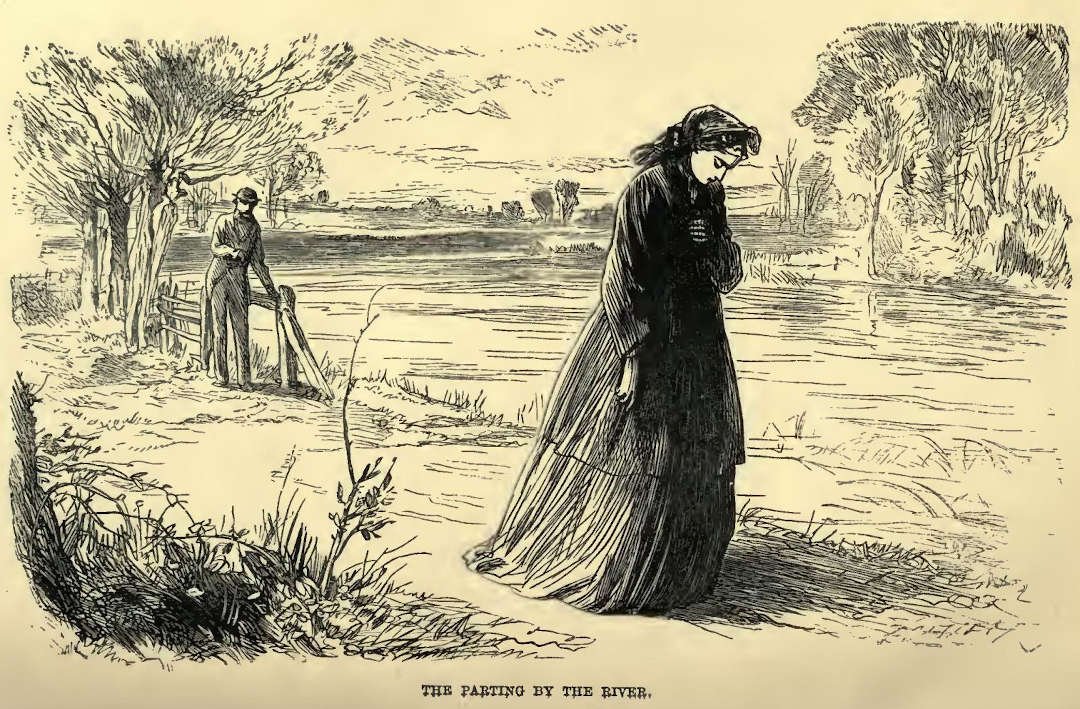
\includegraphics[scale=2.3]{04-06-01}

‘Now, could Mortimer believe this?’ murmured Eugene, still remaining,
after a while, where she had left him. ‘Can I even believe it myself?’

He referred to the circumstance that there were tears upon his hand,
as he stood covering his eyes. ‘A most ridiculous position this, to be
found out in!’ was his next thought. And his next struck its root in a
little rising resentment against the cause of the tears.

‘Yet I have gained a wonderful power over her, too, let her be as much
in earnest as she will!’

The reflection brought back the yielding of her face and form as she
had drooped under his gaze. Contemplating the reproduction, he seemed
to see, for the second time, in the appeal and in the confession of
weakness, a little fear.

‘And she loves me. And so earnest a character must be very earnest in
that passion. She cannot choose for herself to be strong in this fancy,
wavering in that, and weak in the other. She must go through with her
nature, as I must go through with mine. If mine exacts its pains and
penalties all round, so must hers, I suppose.’

Pursuing the inquiry into his own nature, he thought, ‘Now, if I married
her. If, outfacing the absurdity of the situation in correspondence with
M. R. F., I astonished M. R. F. to the utmost extent of his respected
powers, by informing him that I had married her, how would M. R. F.
reason with the legal mind? “You wouldn’t marry for some money and some
station, because you were frightfully likely to become bored. Are you
less frightfully likely to become bored, marrying for no money and no
station? Are you sure of yourself?” Legal mind, in spite of forensic
protestations, must secretly admit, “Good reasoning on the part of M. R.
F. NOT sure of myself.”’

In the very act of calling this tone of levity to his aid, he felt it to
be profligate and worthless, and asserted her against it.

‘And yet,’ said Eugene, ‘I should like to see the fellow (Mortimer
excepted) who would undertake to tell me that this was not a real
sentiment on my part, won out of me by her beauty and her worth,
in spite of myself, and that I would not be true to her. I should
particularly like to see the fellow to-night who would tell me so, or
who would tell me anything that could be construed to her disadvantage;
for I am wearily out of sorts with one Wrayburn who cuts a sorry figure,
and I would far rather be out of sorts with somebody else. “Eugene,
Eugene, Eugene, this is a bad business.” Ah! So go the Mortimer
Lightwood bells, and they sound melancholy to-night.’

Strolling on, he thought of something else to take himself to task for.
‘Where is the analogy, Brute Beast,’ he said impatiently, ‘between a
woman whom your father coolly finds out for you and a woman whom you
have found out for yourself, and have ever drifted after with more and
more of constancy since you first set eyes upon her? Ass! Can you reason
no better than that?’

But, again he subsided into a reminiscence of his first full knowledge
of his power just now, and of her disclosure of her heart. To try no
more to go away, and to try her again, was the reckless conclusion it
turned uppermost. And yet again, ‘Eugene, Eugene, Eugene, this is a bad
business!’ And, ‘I wish I could stop the Lightwood peal, for it sounds
like a knell.’

Looking above, he found that the young moon was up, and that the stars
were beginning to shine in the sky from which the tones of red and
yellow were flickering out, in favour of the calm blue of a summer
night. He was still by the river-side. Turning suddenly, he met a man,
so close upon him that Eugene, surprised, stepped back, to avoid a
collision. The man carried something over his shoulder which might
have been a broken oar, or spar, or bar, and took no notice of him, but
passed on.

‘Halloa, friend!’ said Eugene, calling after him, ‘are you blind?’

The man made no reply, but went his way.

Eugene Wrayburn went the opposite way, with his hands behind him and his
purpose in his thoughts. He passed the sheep, and passed the gate, and
came within hearing of the village sounds, and came to the bridge. The
inn where he stayed, like the village and the mill, was not across
the river, but on that side of the stream on which he walked. However,
knowing the rushy bank and the backwater on the other side to be a
retired place, and feeling out of humour for noise or company, he
crossed the bridge, and sauntered on: looking up at the stars as they
seemed one by one to be kindled in the sky, and looking down at the
river as the same stars seemed to be kindled deep in the water. A
landing-place overshadowed by a willow, and a pleasure-boat lying moored
there among some stakes, caught his eye as he passed along. The spot was
in such dark shadow, that he paused to make out what was there, and then
passed on again.

The rippling of the river seemed to cause a correspondent stir in his
uneasy reflections. He would have laid them asleep if he could, but they
were in movement, like the stream, and all tending one way with a strong
current. As the ripple under the moon broke unexpectedly now and then,
and palely flashed in a new shape and with a new sound, so parts of
his thoughts started, unbidden, from the rest, and revealed their
wickedness. ‘Out of the question to marry her,’ said Eugene, ‘and out of
the question to leave her. The crisis!’

He had sauntered far enough. Before turning to retrace his steps, he
stopped upon the margin, to look down at the reflected night. In an
instant, with a dreadful crash, the reflected night turned crooked,
flames shot jaggedly across the air, and the moon and stars came
bursting from the sky.

Was he struck by lightning? With some incoherent half-formed thought
to that effect, he turned under the blows that were blinding him and
mashing his life, and closed with a murderer, whom he caught by a red
neckerchief--unless the raining down of his own blood gave it that hue.

Eugene was light, active, and expert; but his arms were broken, or he
was paralysed, and could do no more than hang on to the man, with his
head swung back, so that he could see nothing but the heaving sky. After
dragging at the assailant, he fell on the bank with him, and then there
was another great crash, and then a splash, and all was done.

Lizzie Hexam, too, had avoided the noise, and the Saturday movement of
people in the straggling street, and chose to walk alone by the water
until her tears should be dry, and she could so compose herself as
to escape remark upon her looking ill or unhappy on going home. The
peaceful serenity of the hour and place, having no reproaches or evil
intentions within her breast to contend against, sank healingly into
its depths. She had meditated and taken comfort. She, too, was turning
homeward, when she heard a strange sound.

It startled her, for it was like a sound of blows. She stood still, and
listened. It sickened her, for blows fell heavily and cruelly on the
quiet of the night. As she listened, undecided, all was silent. As she
yet listened, she heard a faint groan, and a fall into the river.

Her old bold life and habit instantly inspired her. Without vain waste
of breath in crying for help where there were none to hear, she ran
towards the spot from which the sounds had come. It lay between her and
the bridge, but it was more removed from her than she had thought; the
night being so very quiet, and sound travelling far with the help of
water.

At length, she reached a part of the green bank, much and newly trodden,
where there lay some broken splintered pieces of wood and some torn
fragments of clothes. Stooping, she saw that the grass was bloody.
Following the drops and smears, she saw that the watery margin of the
bank was bloody. Following the current with her eyes, she saw a bloody
face turned up towards the moon, and drifting away.

Now, merciful Heaven be thanked for that old time, and grant, O Blessed
Lord, that through thy wonderful workings it may turn to good at last!
To whomsoever the drifting face belongs, be it man’s or woman’s, help
my humble hands, Lord God, to raise it from death and restore it to some
one to whom it must be dear!

It was thought, fervently thought, but not for a moment did the prayer
check her. She was away before it welled up in her mind, away, swift
and true, yet steady above all--for without steadiness it could never
be done--to the landing-place under the willow-tree, where she also had
seen the boat lying moored among the stakes.

A sure touch of her old practised hand, a sure step of her old practised
foot, a sure light balance of her body, and she was in the boat. A
quick glance of her practised eye showed her, even through the deep dark
shadow, the sculls in a rack against the red-brick garden-wall. Another
moment, and she had cast off (taking the line with her), and the boat
had shot out into the moonlight, and she was rowing down the stream as
never other woman rowed on English water.

Intently over her shoulder, without slackening speed, she looked ahead
for the driving face. She passed the scene of the struggle--yonder it
was, on her left, well over the boat’s stern--she passed on her right,
the end of the village street, a hilly street that almost dipped into
the river; its sounds were growing faint again, and she slackened;
looking as the boat drove, everywhere, everywhere, for the floating
face.

She merely kept the boat before the stream now, and rested on her oars,
knowing well that if the face were not soon visible, it had gone down,
and she would overshoot it. An untrained sight would never have seen by
the moonlight what she saw at the length of a few strokes astern. She
saw the drowning figure rise to the surface, slightly struggle, and as
if by instinct turn over on its back to float. Just so had she first
dimly seen the face which she now dimly saw again.

Firm of look and firm of purpose, she intently watched its coming on,
until it was very near; then, with a touch unshipped her sculls, and
crept aft in the boat, between kneeling and crouching. Once, she let the
body evade her, not being sure of her grasp. Twice, and she had seized
it by its bloody hair.

It was insensible, if not virtually dead; it was mutilated, and streaked
the water all about it with dark red streaks. As it could not help
itself, it was impossible for her to get it on board. She bent over the
stern to secure it with the line, and then the river and its shores rang
to the terrible cry she uttered.

But, as if possessed by supernatural spirit and strength, she lashed
it safe, resumed her seat, and rowed in, desperately, for the nearest
shallow water where she might run the boat aground. Desperately, but not
wildly, for she knew that if she lost distinctness of intention, all was
lost and gone.

She ran the boat ashore, went into the water, released him from the
line, and by main strength lifted him in her arms and laid him in the
bottom of the boat. He had fearful wounds upon him, and she bound them
up with her dress torn into strips. Else, supposing him to be still
alive, she foresaw that he must bleed to death before he could be landed
at his inn, which was the nearest place for succour.

This done very rapidly, she kissed his disfigured forehead, looked up
in anguish to the stars, and blessed him and forgave him, ‘if she had
anything to forgive.’ It was only in that instant that she thought of
herself, and then she thought of herself only for him.

Now, merciful Heaven be thanked for that old time, enabling me, without
a wasted moment, to have got the boat afloat again, and to row back
against the stream! And grant, O Blessed Lord God, that through poor me
he may be raised from death, and preserved to some one else to whom he
may be dear one day, though never dearer than to me!

She rowed hard--rowed desperately, but never wildly--and seldom removed
her eyes from him in the bottom of the boat. She had so laid him there,
as that she might see his disfigured face; it was so much disfigured
that his mother might have covered it, but it was above and beyond
disfigurement in her eyes.

The boat touched the edge of the patch of inn lawn, sloping gently to
the water. There were lights in the windows, but there chanced to be
no one out of doors. She made the boat fast, and again by main strength
took him up, and never laid him down until she laid him down in the
house.

Surgeons were sent for, and she sat supporting his head. She had
oftentimes heard in days that were gone, how doctors would lift the hand
of an insensible wounded person, and would drop it if the person were
dead. She waited for the awful moment when the doctors might lift this
hand, all broken and bruised, and let it fall.

The first of the surgeons came, and asked, before proceeding to his
examination, ‘Who brought him in?’

‘I brought him in, sir,’ answered Lizzie, at whom all present looked.

‘You, my dear? You could not lift, far less carry, this weight.’

‘I think I could not, at another time, sir; but I am sure I did.’

The surgeon looked at her with great attention, and with some
compassion. Having with a grave face touched the wounds upon the head,
and the broken arms, he took the hand.

O! would he let it drop?

He appeared irresolute. He did not retain it, but laid it gently down,
took a candle, looked more closely at the injuries on the head, and at
the pupils of the eyes. That done, he replaced the candle and took the
hand again. Another surgeon then coming in, the two exchanged a whisper,
and the second took the hand. Neither did he let it fall at once, but
kept it for a while and laid it gently down.

‘Attend to the poor girl,’ said the first surgeon then. ‘She is quite
unconscious. She sees nothing and hears nothing. All the better for
her! Don’t rouse her, if you can help it; only move her. Poor girl, poor
girl! She must be amazingly strong of heart, but it is much to be feared
that she has set her heart upon the dead. Be gentle with her.’



